\section{Auto-encoders}
Bir veri setindeki gizli yapıyı öğrenmek ve ardından veriyi bu gizli yapıyı kullanarak yeniden oluşturmak için kullanılır. Bu işlem, veri sıkıştırma ve ardından sıkıştırılmış veriden orijinal veriyi geri oluşturma olarak düşünülebilir. Bir autoencoder, genellikle iki bölümden oluşur:
\begin{enumerate}
    \item \textbf{Encoder (Kodlayıcı):} Giriş verisini daha düşük boyutlu bir temsile dönüştüren kısmıdır.
    \item \textbf{Decoder (Çözücü):} Kodlayıcı tarafından oluşturulan kodu alır ve orijinal giriş verisini yeniden oluşturmak için kullanır. 
\end{enumerate}

\begin{figure}[h]
    \centering
    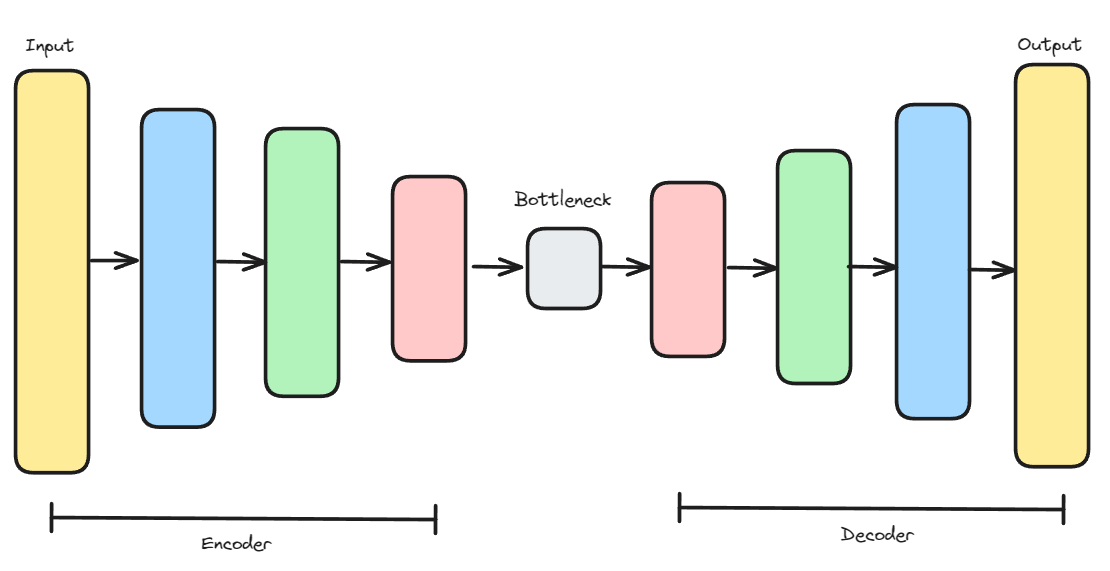
\includegraphics[width=1\textwidth]{images/autoencoder_architecture.png}
    \caption{Auto-encoder mimarisi.}
    \label{fig:enter-label}
\end{figure}

\subsection{Çalışma Adımları}
Giriş veri bir vektör olarak temsil edilir. Encoder ağı, bu giriş veriyi alan ve daha düşük boyutlu bir kod temsilini dönüştüren bir dizi katmandan oluşur. Her katman, giriş verisini daha soyut ve düşük boyutlu bir şekilde temsil eden özellikler çıkarır. Encoder ve Decoder ağları arasında bir Bottleneck (darboğaz) katmanı bulunur. Bottleneck katmanı, elde edilecek kodun büyüklüğünü (ne kadar sıkıştırma yapılacağını) belirler. Bottleneck katmanının çıktısı, kod veya latent vector olarak adlandırılan daha küçük boyutlu bir vektördür. Bu kod, giriş verisinin temsilidir. Decoder ağı, kodu alır ve orijinal giriş verisini yeniden oluşturmak için kullanılır. Decoder, kodu daha yüksek boyutlu bir vektöre dönüştürür ve orijinal giriş verisinin yapılandırılmasını sağlar. Autoencoder'in eğitimi, yeniden yapılandırılan çıktının orijinal girişe ne kadar yakın olduğunu ölçen bir kayıp fonksiyonunu minimize etmeye dayanır. 

\subsection{Sıkıştırma Türleri}
\begin{itemize}
    \item \textbf{Kayıplı Sıkıştırma (Lossy Compression):} Kayıplı sıkıştırma, veri boyutunu azaltırken orijinal verinin tam olarak yeniden elde edilememesi anlamına gelir. Bu, sıkıştırma esnasında bazı bilgilerin kaybolacağı anlamına gelir. Autoencoder'lar kayıplı sıkıştırmayı kullanır. Veriyi en az kayıpla sıkıştıracak şekilde eğitilir. Veriyi kayıpsız olarak sıkıştırma teorik olarak mümkün olsa da bu hep kullanım amacına aykırıdır hem de verimliliğinin azalmasına ve overfitting problemlerine neden olur. 
    \item \textbf{Kayıpsız Sıkıştırma (Lossless Compression):} Kayıpsız sıkılaştırma, veri boyutunu azaltırken orijinal veriyi tam olarak yeniden elde edebilme yeteneği sağlar. Bu, sıkıştırma esnasından hiçbir bilginin kaybolmayacağı anlamına gelir.
\end{itemize}

\subsection{Kullanım Alanları}
\begin{itemize}
    \item \textbf{Feature Extraction (Özellik Çıkarma)} Autoencoder'lar verideki en önemli noktaları tuttukları için özellik çıkarımında kullanılabilirler.
    \item \textbf{Dimension Reduction (Boyut Azaltma)}
    \item \textbf{Denoising (Gürültü Azaltma)}
    \item \textbf{Anomali Tespiti}
    \item \textbf{Yeni Veri Üretme}
    \item \textbf{Resim Tamamlama veya Renklendirme}
\end{itemize}

\subsection{Türleri}
\begin{itemize}
    \item \textbf{Vanilla Autoencoder:} Temel ve basit formdaki autoencoder türüdür. "Vanilla", temel anlamına gelir. Bu basit mimari genellikle tam bağlı (fully connected) katmanlardan oluşur.
    \item \textbf{Denoising Autoencoder:} Veri setindeki gürültüyü temizlemek için kullanılır. Gürültülü bir giriş verisi alır ve bu gürültülü veriyi gürültüsüz orijinal veriye daha yakın bir temsil ile yeniden oluşturmayı amaçlar. 
    \item \textbf{Convolutional Autoencoder:} CNN mimarisinden esinlenerek tasarlanıştır. Encoder, convolutional katmanlar kullanarak giriş verisini işler. Convolutional Encoder, üretilen özellik haritalarını düzleştirerek ve daha sonra tam bağlantılı katmanlar kullanarak bir kod temsili oluşturur. Convolutional Decoder, tam bağlantılı katmanlar ve ters konvolüsyonel (deconv) katmanmları kullanarak kodu daha yüksek boyutlu bir vektöre dönüştürür ve orijinal giriş verisini yeniden yapılandırır.
    \item \textbf{Variational Autoencoder:} İstatistiksel ve generative bir autoencoder türüdür. VAE, diğer autoencoder türlerinden farklı olarak, verinin latent uzayında bir olasılık dağılımını öğrenir ve bu dağılımdan örnekler çıkararak yeni veri örnekleri üretme yeteneğine sahiptir. VAE'de encoder çıktısı bir kod değil giriş verisini temsil eden bir ortalama vektörü ve varyans vektörüdür. Encoder, bu vektörleri ürettikten sonra bu dağılıma göre bir nokta seçmek için bir örnekleme işlemi gerçekleştirilir. Decoder, örnekleme işleminden elde edilen noktayı alır ve orijinal giriş verisini yeniden oluşturmak için kullanılır. VAE'nin kayıp fonksiyonu Kullback-Leibler (KL) Divergence içerir. KL Divergence, iki olasılık dağılımı arasındaki farkı ölçer. Model tarafından öğrenilen olasılık dağılımının gerçek veri dağılımına ne kadar yakın olduğunu değerlendirmek için kullanılır.
    \item \textbf{Recurrent Autoencoder:} Zaman serisi veri setleriyle kullanılır. Giriş verisinin zaman bağlamını koruyarak sıkıştırma ve yeniden yapılandırma işlemlerini gerçekleştirir. 
    \item \textbf{Sparse Autoencoder:} Giriş verisindeki özelliklerin daha az sayıda nöron tarafından temsil edilmesini sağlar. Giriş verisindeki özelliklerin özünü daha etkin bir şekilde temsil etmesini ve gereksiz özelliklerin bastırılmasını amaçlar. Sparse regularizasyon içerir.
    \item \textbf{Contractive Autoencoder:} Giriş verisini daha küçük boyutlu bir kod temsiline sıkıştırırken, veri uzayındaki konumları birleştirir ve bu sayede modelin giriş verisinin çeşitli varyasyonlarına karşı daha dirençli hale gelmesini sağlar. Contractive regularizasyon içerir.
    \item \textbf{Fully Connected Autoencoder:} Giriş verisini düzleştirerek ve tam bağlantılı katmanlar aracılığıyla sıkıştırma ve yeniden yapılandırma işlemlerini gerçekleştirir. Diğer autoencoder türlerinden farkı, özellikle görüntü verileri gibi yapısal verilerle çalışırken, zaman serileri veya metin verileri gibi veri yapılarını işlemek için tekrarlayan katmanlar gibi özel yapıları içermez.
\end{itemize}

\subsection{Python Kodu}

\begin{lstlisting}[language=Python]
class VAE(nn.Module):
    def __init__(self, input_dim, hidden_dim, latent_dim):
        super(VAE, self).__init__()
        self.fc1 = nn.Linear(input_dim, hidden_dim)
        self.fc2_mu = nn.Linear(hidden_dim, latent_dim)
        self.fc2_logvar = nn.Linear(hidden_dim, latent_dim)
        self.fc3 = nn.Linear(latent_dim, hidden_dim)
        self.fc4 = nn.Linear(hidden_dim, input_dim)

    def encode(self, x):
        h1 = torch.relu(self.fc1(x))
        return self.fc2_mu(h1), self.fc2_logvar(h1)

    def reparameterize(self, mu, logvar):
        std = torch.exp(0.5 * logvar)
        eps = torch.randn_like(std)
        return mu + eps * std

    def decode(self, z):
        h3 = torch.relu(self.fc3(z))
        return torch.sigmoid(self.fc4(h3))

    def forward(self, x):
        mu, logvar = self.encode(x.view(-1, 784))
        z = self.reparameterize(mu, logvar)
        return self.decode(z), mu, logvar

def loss_function(recon_x, x, mu, logvar):
    BCE = F.mse_loss(recon_x, x.view(-1, 784), reduction='sum')
    KLD = -0.5 * torch.sum(1 + logvar - mu.pow(2) - logvar.exp())
    return BCE + KLD

input_dim = 784
hidden_dim = 400
latent_dim = 50

model = VAE(input_dim, hidden_dim, latent_dim).to(device)

lr = 1e-3
optimizer = optim.Adam(model.parameters(), lr=lr)
n_epochs = 10

def train_batch(data, model, optimizer, loss_function):
    model.train()
    data = data.to(device)
    optimizer.zero_grad()
    recon_batch, mean, log_var = model(data)
    
    loss = loss_function(recon_batch, data, mean, log_var)
    loss.backward()
    optimizer.step()
    return loss.item()

@torch.no_grad()
def validate_batch(data, model, loss_function):
    model.eval()
    data = data.to(device)
    recon, mean, log_var = model(data)
    loss = loss_function(recon, data, mean, log_var)
    return loss.item()

train_losses = []
valid_losses = []

for epoch in range(n_epochs):
    model.train()
    for batch_idx, (data, _) in enumerate(train_dataloader):
        train_loss = train_batch(data, model, optimizer, loss_function)
        train_losses.append(train_loss)
        if batch_idx % 200 == 0:
            print(f"Epoch [{epoch+1}/{n_epochs}], Batch [{batch_idx+1}/{len(train_dataloader)}], Train Loss: {train_loss}")
        
    model.eval()
    with torch.no_grad():
        for batch_idx, (data, _) in enumerate(test_dataloader):
            valid_loss = validate_batch(data, model, loss_function)
            valid_losses.append(valid_loss)
            if batch_idx % 200 == 0:
                print(f"Epoch [{epoch+1}/{n_epochs}], Batch [{batch_idx+1}/{len(test_dataloader)}], Valid Loss: {valid_loss}")
\end{lstlisting}

\newpage